\section{Theorie}
\label{sec:Theorie}

% In knapper Form sind die physikalischen Grundlagen des Versuches, des Messverfahrens, sowie sämtliche für die Auswertung erforderlichen Gleichungen darzustellen. (Keine Herleitung)

% (eventuell die Aufgaben)

% Der Versuchsaufbau: Beschreibung des Versuchs und der Funktionsweise (mit Skizze/Bild/Foto)

\begin{figure}
    \centering
    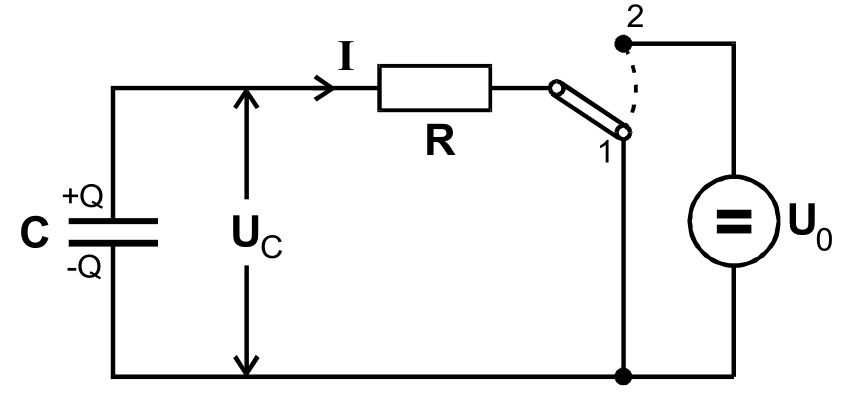
\includegraphics[width=\textwidth/2]{images/schaltung_1.png}
    \caption{Schaltbild eines RC-Kreises, der in Stellung 1 entladen und in Stellung 2 geladen wird. \cite{V353}}
    \label{fig:schaltung_1}
\end{figure}

Wenn ein System durch eine Änderung aus seinem Anfangszustand entfernt wird und daraufhin nicht-oszillatorisch in diesen zurückkehrt, kann man Relaxationseffekte beobachten. In \autoref{fig:schaltung_1} sind zwei dieser Relaxationsphänomene zu beobachten, das Auf- und Entladen eines Kondensators über einen Widerstand. 
Befindet sich der Schalter in \autoref{fig:schaltung_1} in Stellung eins, so entlädt sich der Kondensator mit der Kapazität $C$. Auf seinen beiden Platten liegt die Ladung Gesamtladung $Q$. Dadurch liegt zwischen den beiden Kondensatorplatten eine Spannung von 

\begin{equation}
    \label{eq:kondensatorspannung}
    U_C = \frac{Q}{C}.
\end{equation}

Durch das ohmsche Gesetz ist bekannt, dass durch diese Spannung $U_C$ und den Widerstand $R$ ein Strom 

\begin{equation}
    \label{eq:ohmschesgesetz}
    I = \frac{U_C}{R}
\end{equation}

erzeugt wird. 
Der zeitliche Verlauf der Ladung $Q$ auf dem Kondensator $C$ kann durch eine Exponentialfunktion beschrieben werden, dadurch ergibt sich

\begin{equation}
    \label{eq:entladungsladung}
    Q (t) = Q (0) \exp{\left(\frac{-t}{RC} \right)}.
\end{equation}

Wobei $RC$ eine Zeitkonstante ist, die im nächsten Abschnitt näher erklärt wird. \cite{V353}
Äquivalent dazu lässt sich der Aufladevorgang eines Kondensators $C$ durch die Spannung $U_0$ über den Widerstand $R$ beschreiben. Hierbei gelten folgende Randbedingungen für $Q$

\begin{align}
    \label{eq:ladung}
    Q (0) = 0 && Q (\infty) = C \cdot U_0.
\end{align}

Damit lässt sich der Aufladevorgang durch

\begin{equation}
    \label{eq:aufladungsladung}
    Q (t) = C \cdot U_0  (1- \exp{\left(\frac{-t}{RC} \right)} )
\end{equation}

beschreiben. \cite{V353} Dabei ist $RC$ wieder die Zeitkonstante aus \autoref{entladungsladung}, mit dieser Konstante kann beschrieben werden, wie schnell sich ein System zu seinem Endzustand begibt. $RC$ ist festgeschrieben. Nachdem eine Zeit von 
\begin{equation}
    \Delta T = RC
\end{equation} verstrichen ist, ändert sich die Kondensatorladung $Q$ um den Faktor
\begin{equation}
    \label{eq:RC}
    \frac{Q (t = RC)}{Q (0)} = \frac{1}{e} \approx 0.386.
\end{equation}

\begin{figure}
    \centering
    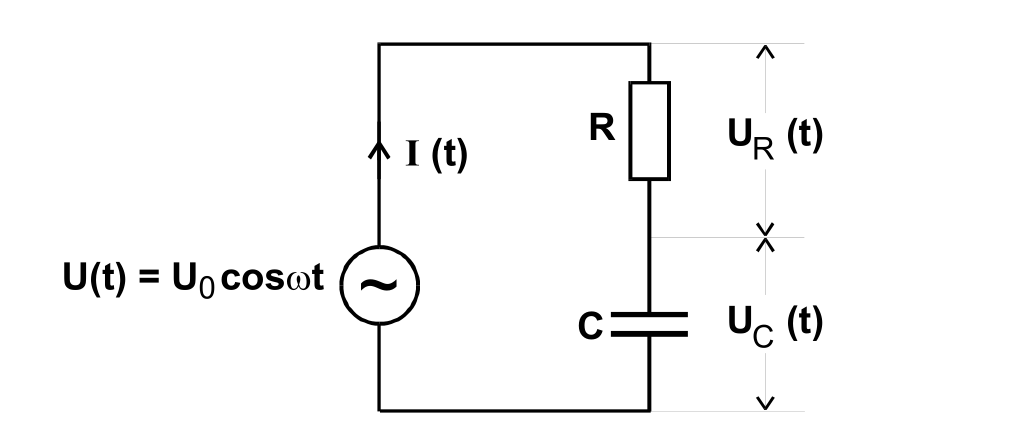
\includegraphics[width=\textwidth/2]{images/schaltung_2.png}
    \caption{Mögliches Schaltbild zur Entstehung eines Relaxationsphänomens durch periodische Anregung.  \cite{V353}}
    \label{fig:schaltung_2}
\end{figure}